\chapter{الأطياف الإلكترونية للمعقدات ومغناطيسيتها}\label{ch:b3:complex-spectra-magnetism}

الياقوت أحمر والزمرد أخضر، ومع ذلك يدين كلاهما بلونه للأيون نفسه،
\ce{Cr^{3+}}، الذي يحل محل بضعة أيونات ألومنيوم في أكسيدين مختلفين: الكوراندوم،
$\ce{Al2O3}$، في الياقوت، وسيليكات البيريليوم والألومنيوم المسماة بيريل في الزمرد. وفي
كليهما يجلس الكروم في ثماني أوجه من ذرات الأكسجين؛ وفي البيريل يكون
ثماني الأوجه أكبر قليلًا ومجال الربائط أضعف قليلًا، فتنزاح
حزم امتصاص الأيون بنحو ألف عدد موجي نحو الأحمر.
وهذا يكفي لتغيير اللون النافذ من الأحمر إلى الأخضر. ويفسّر هذا الفصل
مثل هذه الأطياف كميًا: كيف تنشطر حدود الأيون الحر في
مجال الربائط، وكيف تحوّل \omterm{def:b3:complex-spectra-magnetism:tanabe-sugano}{مخططات تانابه--سوغانو} موضعي حزمتين إلى
انشطار مجال الربائط وإلى التنافر الإلكتروني، ولماذا تكون بعض الحزم شديدة
وأخرى خافتة، ولماذا تتشوه بعض المعقدات، وكيف تعدّ المغناطيسية
الإلكترونات المنفردة.

\begin{recall}
عالج مجلد السنة الثانية العناصر الانتقالية وتشكيلاتها $d^n$، 
وانشطار المجال البلوري $\Delta_{\mathrm o}$، والمعقدات عالية السبين ومنخفضة السبين، وطاقة الاقتران، 
وطاقة استقرار المجال البلوري، وانتقالات \babelsublr{$d$--$d$}، والسلسلة الطيفية
الكيميائية، ونظرية مجال الربائط، والمواد البارامغناطيسية والديامغناطيسية.
واشتق \cref{ch:b3:many-electron-atoms} رموز الحدود وقواعد هوند،
واختزل \cref{ch:b3:group-theory-applied} التمثيلات والجداءات المباشرة،
وذكر \cref{ch:b3:electronic-spectroscopy} قاعدتي انتقاء السبين ولابورت
ووصف انتقالات نقل الشحنة، 
وأعطى \cref{ch:b3:partition-functions} \omterm{def:b3:partition-functions:boltzmann}{توزيع بولتزمان}.
\end{recall}

\begin{omfigure}
\begin{minipage}[b]{0.3\linewidth}\centering
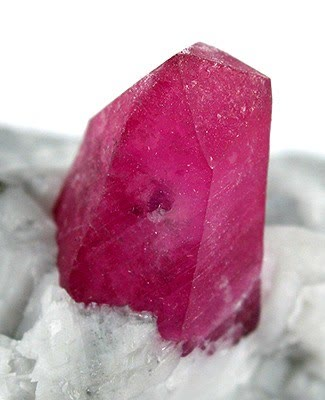
\includegraphics[height=4.2cm]{images/book4/ruby-crystal.jpg}\par
{\small ياقوت}
\end{minipage}\hspace{1.5em}
\begin{minipage}[b]{0.3\linewidth}\centering
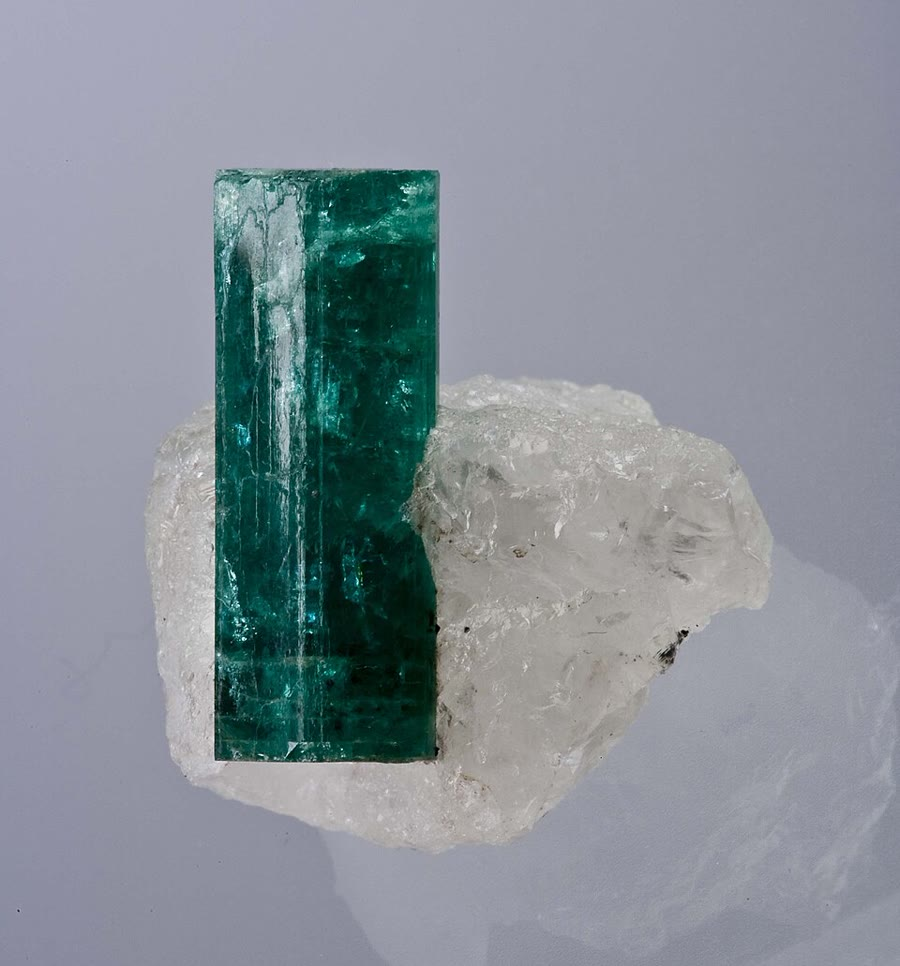
\includegraphics[height=4.2cm]{images/book4/emerald-crystal.jpg}\par
{\small زمرد}
\end{minipage}

{\small بلورة ياقوت في الرخام وبلورة زمرد على الكوارتز. وفي كلتيهما يأتي
اللون من بضعة في المئة من \ce{Cr^{3+}} في موقع ثماني الأوجه.}
\end{omfigure}

\section{من حدود الأيون الحر إلى حدود مجال الربائط}

في الأيون الحر يشطر التنافر الإلكتروني التشكيل $d^n$ إلى حدود
(\babelsublr{$^4$F} و\babelsublr{$^4$P} و\babelsublr{$^2$G}\dots\ من أجل $d^3$، \cref{ch:b3:many-electron-atoms}). وفي المعقد، ينشطر كل حد
أيضًا بفعل الربائط، وتُوسم المستويات \omterm{def:b3:point-groups:irrep}{بالتمثيلات غير القابلة للاختزال}
\omterm{def:b3:point-groups:point-group}{للزمرة النقطية} للمعقد.

\begin{definition}[حد مجال الربائط]\label{def:b3:complex-spectra-magnetism:ligand-field-term}
\emph{حد مجال الربائط}\index{حد مجال الربائط} لمعقد مجموعة من
الحالات المتعددة الإلكترونات المنحلة، توسم بتعددية سبينها 
وبالتمثيل غير القابل للاختزال \omterm{def:b3:point-groups:point-group}{للزمرة النقطية} الذي ينتمي إليه جزؤها المداري،
مثل \babelsublr{$^4$A$_{2g}$} أو \babelsublr{$^4$T$_{1g}$} في معقد ثماني الأوجه.
\end{definition}

\begin{proposition}[مميِّزات زمرة الدورانات]\label{prop:b3:complex-spectra-magnetism:rotation-characters}
تكوّن الحالات $2L+1$ لحد زخمه الزاوي المداري $L$ تمثيلًا
لزمرة الدورانات مميِّزه من أجل دوران بزاوية $\alpha$ هو
\[
  \chi_L(\alpha) = \frac{\sin\bigl((L + \tfrac12)\alpha\bigr)}{\sin(\alpha/2)}, \qquad \chi_L(0) = 2L + 1 .
\]
\end{proposition}

\admitted

\begin{theorem}[انشطار حدود الأيون الحر في مجال ثماني الأوجه]\label{thm:b3:complex-spectra-magnetism:term-splitting}
في مجال ثماني الأوجه تنشطر حدود الأيون $d^n$ إلى
\begin{center}
\begin{tabular}{ll}
\hline
حد الأيون الحر & حدود ثماني الأوجه (\omterm{def:b3:many-electron-atoms:term}{بتعددية السبين} نفسها) \\ \hline
S & \babelsublr{A$_{1g}$} \\
P & \babelsublr{T$_{1g}$} \\
D & \babelsublr{E$_g$ + T$_{2g}$} \\
F & \babelsublr{A$_{2g}$ + T$_{1g}$ + T$_{2g}$} \\
G & \babelsublr{A$_{1g}$ + E$_g$ + T$_{1g}$ + T$_{2g}$} \\ \hline
\end{tabular}
\end{center}
\end{theorem}

\begin{proof}
زمرة ثماني الأوجه هي زمرة الدورانات $O$ مضروبة في الانقلاب؛ والدوال $d$
زوجية، فكل حد من حدود التشكيل $d^n$ زوجي ($g$)، ويكفي
الاختزال في $O$، التي أصنافها $E$ و$8C_3$ و$3C_2$ ($=C_4^2$) و$6C_4$ و$6C_2'$. وبالقضية،
من أجل $L = 3$: $\chi = 7$، $\sin(420^\circ)/\sin60^\circ = 1$، $\sin(630^\circ)/\sin90^\circ = -1$، $\sin(315^\circ)/\sin45^\circ = -1$
و$-1$. ويعطي جدول \omterm{def:b3:point-groups:representation}{مميِّزات} $O$ (الصفوف $A_1$: 1، 1، 1، 1، 1؛ $A_2$: 1، 1، 1، $-1$، $-1$؛ $E$: 2،
$-1$، 2، 0، 0؛ $T_1$: 3، 0، $-1$، 1، $-1$؛ $T_2$: 3، 0، $-1$، $-1$، 1) \omterm{thm:b3:group-theory-applied:reduction}{وصيغة الاختزال} في
\cref{ch:b3:group-theory-applied} القيم $n(A_2) = (7 + 8 - 3 + 6 + 6)/24 = 1$، $n(T_1) = (21 + 3 - 6 +
6)/24 = 1$، $n(T_2) = (21 + 3 + 6 - 6)/24 = 1$، والصفر من أجل $A_1$ و$E$. وتُستخرج الصفوف الأخرى
بالطريقة نفسها ($L = 0$: $(1, 1, 1, 1, 1)$؛ $L = 1$: $(3, 0, -1, 1, -1)$؛ $L = 2$: $(5, -1, 1,
-1, 1)$؛ $L = 4$: $(9, 0, 1, 1, 1)$).
\end{proof}

\begin{method}[شطر حد للأيون الحر]\label{met:b3:complex-spectra-magnetism:split-term}
\begin{enumerate}
  \item أوجد الحد الأساسي للأيون الحر (قواعد هوند) والحدود المثارة
        ذات التعددية نفسها.
  \item اقرأ مركّباتها في ثماني الأوجه في الجدول؛ \omterm{def:b3:many-electron-atoms:term}{وتعددية السبين}
        لا تتغير.
  \item رتّبها: من أجل الحد الأساسي F للتشكيلين $d^2$ و$d^7$ (عالي السبين) يكون الأدنى \babelsublr{T$_{1g}$}؛
        ومن أجل $d^3$ و$d^8$ يكون \babelsublr{A$_{2g}$} (القضية التالية).
\end{enumerate}
\end{method}

\begin{proposition}[الثقوب والانقلاب رباعي الأوجه]\label{prop:b3:complex-spectra-magnetism:hole}
حدود $d^{10-n}$ في مجال ثماني الأوجه هي حدود $d^n$ بترتيب طاقي
معكوس؛ وحدود $d^n$ في مجال رباعي الأوجه هي حدود $d^{10-n}$ في مجال ثماني
الأوجه (مع حذف الأدلة $g$).
\end{proposition}

\begin{proof}
التشكيل $d^{10-n}$ مكافئ لعدد $n$ من الثقوب الموجبة في طبقة ممتلئة: 
والثقوب تحس بكمون مجال الربائط بالإشارة المعاكسة، فينعكس كل
انشطار أحادي الإلكترون، ومنه كل انشطار للحدود (
والتنافر الإلكتروني بين الثقوب هو نفسه بين الإلكترونات). والمجال
رباعي الأوجه إشارته معاكسة لإشارة المجال ثماني الأوجه (فالمدارات $e$
أدنى) وليس له مركز تناظر: فيسلك $d^n$ في $T_d$ سلوك $d^n$ في مجال معكوس،
أي سلوك $d^{10-n}$ في $O_h$.
\end{proof}

\begin{definition}[مخطط الترابط]\label{def:b3:complex-spectra-magnetism:correlation}
\emph{مخطط الترابط}\index{مخطط الترابط} يصل حالات
نظام في وضعين حدّيين، هما هنا حدود الأيون الحر التي يشطرها مجال
ضعيف والتشكيلات $t_{2g}^ae_g^b$ لمجال قوي، فيربط بين حالات
التناظر نفسه دون أن يسمح لحالتين منها بالتقاطع.
\end{definition}

\begin{omfigure}
\begin{tikzpicture}[font=\small]
  % free ion
  \pic (F) at (0,0) {omlevel={}{1.1}};
  \pic (P) at (0,3.0) {omlevel={}{1.1}};
  \node[anchor=east] at (F-l) {$^3$F};
  \node[anchor=east] at (P-l) {$^3$P};
  % weak field
  \pic (a) at (2.6,-0.8) {omlevel={}{1.0}};
  \pic (b) at (2.6,0.3) {omlevel={}{1.0}};
  \pic (c) at (2.6,1.4) {omlevel={}{1.0}};
  \pic (d) at (2.6,3.1) {omlevel={}{1.0}};
  \foreach \n/\t in {a/T$_{1g}$, b/T$_{2g}$, c/A$_{2g}$, d/T$_{1g}$(P)}{\node[omsymlabel, anchor=south] at (\n-c) {$^3$\t};}
  \draw[omcorr] (F-r) -- (a-l) (F-r) -- (b-l) (F-r) -- (c-l) (P-r) -- (d-l);
  % strong field configurations
  \pic (A) at (7.4,-1.6) {omlevel={}{1.0}};
  \pic (B) at (7.4,1.4) {omlevel={}{1.0}};
  \pic (C) at (7.4,1.9) {omlevel={}{1.0}};
  \pic (D) at (7.4,4.6) {omlevel={}{1.0}};
  \node[anchor=west] at (A-r) {$^3$T$_{1g}$ \quad $t_{2g}^2$};
  \node[anchor=west] at (B-r) {$^3$T$_{2g}$};
  \node[anchor=west] at (C-r) {$^3$T$_{1g}$ \quad $t_{2g}e_g$};
  \node[anchor=west] at (D-r) {$^3$A$_{2g}$ \quad $e_g^2$};
  \draw[omcorr] (a-r) -- (A-l) (b-r) -- (B-l) (c-r) -- (D-l) (d-r) -- (C-l);
  \node[anchor=north] at (0,-2.0) {\foreignlanguage{arabic}{الأيون الحر}};
  \node[anchor=north] at (2.6,-2.0) {\foreignlanguage{arabic}{مجال ضعيف}};
  \node[anchor=north] at (7.4,-2.0) {\foreignlanguage{arabic}{مجال قوي}};
  \draw[->, black!50] (3.7,-2.3) -- (6.2,-2.3) node[midway, below, font=\scriptsize] {\foreignlanguage{arabic}{تزايد $\Delta_{\mathrm o}$}};
\end{tikzpicture}

{\small \omterm{def:b3:complex-spectra-magnetism:correlation}{مخطط الترابط} للحالات الثلاثية لأيون $d^2$ في مجال
ثماني الأوجه. يذهب كل حد في المجال الضعيف إلى تشكيل المجال القوي ذي
التناظر نفسه، ولا تتقاطع الحالتان \babelsublr{$^3$T$_{1g}$}: فالدنيا تذهب إلى $t_{2g}^2$، والعليا إلى
$t_{2g}e_g$.}
\end{omfigure}

\section{مخططات تانابه--سوغانو}

\begin{definition}[وسائط راكا]\label{def:b3:complex-spectra-magnetism:racah}
\emph{وسائط راكا}\index{وسائط راكا} $A$ و$B$ و$C$ تراكيب من
تكاملات سلاتر للطبقة $d$ تعبّر عن كل طاقات التنافر الإلكتروني
للتشكيل $d^n$؛ وفروق الطاقة بين حدود
التشكيل نفسه لا تتوقف إلا على $B$ و$C$، وتلك التي بين حدود التعددية
العظمى نفسها لا تتوقف إلا على $B$ (من أجل $d^2$ و$d^3$ و$d^7$ و$d^8$: $E(\mathrm P) - E(\mathrm F) = 15B$).
\end{definition}

\begin{example}[وسائط راكا للأيون الحر]\label{ex:b3:complex-spectra-magnetism:free-B}
% ledger: lev:Cr3.4F5_2, lev:Cr3.4F7_2, lev:Cr3.4F9_2, lev:Cr3.4P1_2, lev:Cr3.4P3_2, lev:Cr3.4P5_2, lev:Ni2.3F3, lev:Ni2.3F2, lev:Ni2.3P2, lev:Ni2.3P1, lev:Ni2.3P0, lev:V2.4F5_2, lev:V2.4F7_2, lev:V2.4F9_2, lev:V2.4P1_2, lev:V2.4P3_2, lev:V2.4P5_2
تضع مستويات الأيون الحر \ce{Cr^{3+}} مركز الثقل (بالأوزان $2J + 1$) للحد \babelsublr{$^4$F} عند
\qty{547}{cm^{-1}} ومركز ثقل \babelsublr{$^4$P} عند \qty{14305}{cm^{-1}} فوق المستوى الأساسي: $15B = \qty{13758}{cm^{-1}}$،
$B = \qty{917}{cm^{-1}}$. ويعطي الحساب نفسه $B = 755$ من أجل \ce{V^{2+}} و\qty{1056}{cm^{-1}} من أجل
\ce{Ni^{2+}}.
\end{example}

\begin{definition}[مخطط تانابه--سوغانو]\label{def:b3:complex-spectra-magnetism:tanabe-sugano}
\emph{مخطط تانابه--سوغانو}\index{مخطط تانابه--سوغانو} يرسم طاقات
كل \omterm{def:b3:complex-spectra-magnetism:ligand-field-term}{حدود مجال الربائط} لأيون $d^n$، بوحدة $B$ ومقيسةً من
الحد الأساسي، بدلالة $\Delta_{\mathrm o}/B$، من أجل نسبة ثابتة $C/B$.
\end{definition}

\begin{proposition}[الحزم الثلاث لأيون $d^3$]\label{prop:b3:complex-spectra-magnetism:d3-bands}
من أجل أيون $d^3$ في مجال ثماني الأوجه تقع الانتقالات المسموحة سبينيًا انطلاقًا من \babelsublr{$^4$A$_{2g}$} عند
\[
  \nu_1 = \Delta_{\mathrm o}\ (^4\mathrm T_{2g}), \qquad
  \nu_{2,3} = 7.5B + 1.5\Delta_{\mathrm o} \mp \tfrac12\sqrt{225B^2 - 18B\Delta_{\mathrm o} + \Delta_{\mathrm o}^2}\ (^4\mathrm T_{1g}(\mathrm F), {}^4\mathrm T_{1g}(\mathrm P)).
\]
\end{proposition}

\begin{proof}[برهان جزئي]
في أساس المجال القوي، يظهر \babelsublr{$^4$A$_{2g}$} و\babelsublr{$^4$T$_{2g}$} مرة واحدة لكل منهما، من $t_{2g}^3$ ومن $t_{2g}^2e_g$، 
ولا يحوي الفرق بينهما أي تنافر إلكتروني: $\nu_1 = \Delta_{\mathrm o}$ بالضبط. أما \babelsublr{$^4$T$_{1g}$} فيظهر
مرتين، من $t_{2g}^2e_g$ ومن $t_{2g}e_g^2$؛ ونسبةً إلى \babelsublr{$^4$A$_{2g}$} تكون المصفوفة $2\times2$ هي
\babelsublr{$\begin{pmatrix}\Delta_{\mathrm o} + 12B & 6B\\ 6B & 2\Delta_{\mathrm o} + 3B\end{pmatrix}$} (ونقبل عناصر التنافر الإلكتروني).
وقيمها الذاتية هي جذور $E^2 - (15B + 3\Delta_{\mathrm o})E + 2\Delta_{\mathrm o}^2 + 27B\Delta_{\mathrm o} = 0$، وهي
$\nu_2$ و$\nu_3$ المذكورتان. وعند $\Delta_{\mathrm o} = 0$ تساويان 0 و$15B$ (الحدان \babelsublr{$^4$F} و\babelsublr{$^4$P})؛ 
ويعيدهما التقطير الكامل في الشكل.
\end{proof}

\begin{omfigure}
\begin{tikzpicture}
\begin{axis}[name=ta, omts, width=0.46\linewidth, height=7.0cm, xmin=1, xmax=40, ymin=0, ymax=70,
  xlabel={$\Delta_{\mathrm o}/B$}, ylabel={$E/B$}, title={\small \babelsublr{$d^3$, $C/B = 4.5$}},
  unbounded coords=jump, clip=true, clip mode=individual]
\foreach \c in {f0,f1,f2,f3,f4,f5,f6,f7,f8,f9,f10,f11,f12,f13,f14,f15}{
  \addplot[omtsforbidden, restrict x to domain=1:40] table[x=x, y=\c] {figdata/out/bachelor-3-tanabe-sugano-d3.dat};}
\foreach \c in {a0,a1,a2,a3}{
  \addplot[omDef, thick, restrict x to domain=1:40] table[x=x, y=\c] {figdata/out/bachelor-3-tanabe-sugano-d3.dat};}
\draw[omThm, dashed] (axis cs:29.0,0) -- (axis cs:29.0,70);
\draw[black!70, dashed] (axis cs:27.1,0) -- (axis cs:27.1,70);
\node[font=\scriptsize, omThm, anchor=north west, rotate=90] at (axis cs:29.6,1.5) {\foreignlanguage{arabic}{ياقوت}};
\node[font=\scriptsize, anchor=south west, rotate=90] at (axis cs:26.6,1.5) {\foreignlanguage{arabic}{زمرد}};
% labels outside the frame, at the height where each curve leaves it
\node[font=\scriptsize, omDef, anchor=west, inner sep=1pt] at (axis cs:40,40) {$^4$T$_{2g}$};
\node[font=\scriptsize, omDef, anchor=west, inner sep=1pt] at (axis cs:40,50.9) {$^4$T$_{1g}$};
\node[font=\scriptsize, omDef, anchor=south, inner sep=1pt] at (axis cs:32.8,70) {$^4$T$_{1g}$(P)};
\node[font=\scriptsize, black!60, anchor=west, inner sep=1pt] at (axis cs:40,21.2) {$^2$E$_g$};
\end{axis}
\begin{axis}[at={(ta.east)}, anchor=west, xshift=2.2cm, omts, width=0.46\linewidth, height=7.0cm,
  xmin=1, xmax=40, ymin=0, ymax=70, xlabel={$\Delta_{\mathrm o}/B$}, ylabel={$E/B$},
  title={\small \babelsublr{$d^8$, $C/B = 4.71$}}, unbounded coords=jump, clip=true, clip mode=individual]
\foreach \c in {f0,f1,f2,f3,f4,f5,f6}{
  \addplot[omtsforbidden, restrict x to domain=1:40] table[x=x, y=\c] {figdata/out/bachelor-3-tanabe-sugano-d8.dat};}
\foreach \c in {a0,a1,a2,a3}{
  \addplot[omDef, thick, restrict x to domain=1:40] table[x=x, y=\c] {figdata/out/bachelor-3-tanabe-sugano-d8.dat};}
\node[font=\scriptsize, omDef, anchor=west, inner sep=1pt] at (axis cs:40,40) {$^3$T$_{2g}$};
\node[font=\scriptsize, omDef, anchor=west, inner sep=1pt] at (axis cs:40,50.9) {$^3$T$_{1g}$};
\node[font=\scriptsize, omDef, anchor=south, inner sep=1pt] at (axis cs:32.8,70) {$^3$T$_{1g}$(P)};
\end{axis}
\end{tikzpicture}

{\small \omterm{def:b3:complex-spectra-magnetism:tanabe-sugano}{مخططا تانابه--سوغانو} لأيونين $d^3$ و$d^8$ محسوبان بتقطير
\omterm{def:b3:quantum-model-systems:schrodinger}{مؤثر هاملتون} لمجال الربائط والتنافر الإلكتروني على كل حالات
التشكيل. بالأزرق السميك: حالات تعددية الحالة الأساسية
(الانتقالات المسموحة سبينيًا)؛ وبالرمادي الرفيع: الحالات الأخرى. والحد الأساسي هو
المحور الأفقي (\babelsublr{$^4$A$_{2g}$} من أجل $d^3$، و\babelsublr{$^3$A$_{2g}$} من أجل $d^8$). بالمتقطع: الياقوت والزمرد، موضوعين عند قيمة $\Delta_{\mathrm o}/B$ لحزمتيهما.
والمستوى \babelsublr{$^2$E$_g$} للتشكيل $d^3$ شبه أفقي: فطاقته لا تكاد تتوقف على المجال.}
\end{omfigure}

\begin{method}[قراءة مخطط تانابه--سوغانو]\label{met:b3:complex-spectra-magnetism:read-ts}
\begin{enumerate}
  \item عيّن الحد الأساسي والانتقالات المسموحة سبينيًا (التعددية
        نفسها).
  \item احسب نسبة طاقتي حزمتين، $\nu_2/\nu_1$؛ وأوجد قيمة $\Delta_{\mathrm o}/B$ التي
        يعطي عندها المخطط هذه النسبة.
  \item اقرأ $E/B$ من أجل $\nu_1$ هناك: $B = \nu_1/(E/B)$، ثم $\Delta_{\mathrm o}$. ومن أجل $d^3$ و$d^8$، $\Delta_{\mathrm o} = \nu_1$
        مباشرة وتعطي الصيغة المغلقة $B$ من $\nu_2$.
  \item قارن $B$ بقيمة الأيون الحر (\omterm{def:b3:complex-spectra-magnetism:nephelauxetic}{النسبة النيفيلوكسيتية}) وتحقّق من أن
        الحزمة الثالثة تقع حيث يتنبأ المخطط.
\end{enumerate}
\end{method}

\begin{definition}[المفعول النيفيلوكسيتي]\label{def:b3:complex-spectra-magnetism:nephelauxetic}
\emph{المفعول النيفيلوكسيتي}\index{مفعول نيفيلوكسيتي} («الموسِّع للسحابة») هو
تناقص وسيط راكا $B$ لأيون فلزي في معقد مقارنةً
بالأيون الحر، بسبب انتشار إلكترونات $d$ على
الربائط؛ و\emph{النسبة النيفيلوكسيتية}\index{نسبة نيفيلوكسيتية} هي $\beta =
B_{\text{المعقد}}/B_{\text{الأيون الحر}}$.
\end{definition}

الربائط الأكثر تساهمية في ارتباطها تخفض $B$ أكثر: فقيمة $\beta$ قرب 0.9 من أجل الفلوريد، و0.8
من أجل الماء، ومن 0.6 إلى 0.7 من أجل الأكسيد والهاليدات الأثقل، وأدنى من ذلك أيضًا من أجل الكبريتيد.
وتظهر الانتقالات الممنوعة سبينيًا، بين حدود مختلفة التعددية،
في صورة خطوط ضعيفة، حادة غالبًا.

\section{الشدات ونقل الشحنة}

\begin{definition}[الاقتران الاهتزازي الإلكتروني]\label{def:b3:complex-spectra-magnetism:vibronic-coupling}
\emph{الاقتران الاهتزازي الإلكتروني}\index{اقتران اهتزازي إلكتروني} هو امتزاج الحركة الإلكترونية 
والحركة الاهتزازية: فالاهتزاز غير المتناظر الذي يزيل مركز
تناظر معقد يمزج قليلًا من الطابع الفردي ($u$) في حالاته $d$،
وهذا يجعل انتقالات \babelsublr{$d$--$d$} الممنوعة وفق لابورت مسموحة على نحو ضعيف.
\end{definition}

\begin{proposition}[شدات حزم الامتصاص]\label{prop:b3:complex-spectra-magnetism:intensity-order}
تتزايد معاملات الامتصاص المولية لحزم المعقدات وفق
الترتيب: \babelsublr{$d$--$d$} الممنوعة سبينيًا \babelsublr{$\ll$ $d$--$d$} المسموحة سبينيًا في معقد ذي مركز تناظر \babelsublr{$<$ $d$--$d$}
في معقد رباعي الأوجه $<$ نقل الشحنة.
\end{proposition}

\begin{proof}[تعليل]
بحسب \cref{ch:b3:electronic-spectroscopy}، يكون الانتقال مسموحًا حين يُحفظ
السبين وتتغير الزوجية. وانتقال \babelsublr{$d$--$d$} لا يغيّر الزوجية أبدًا: ففي
معقد ثماني الأوجه لا يستعير شدة إلا عبر \omterm{def:b3:complex-spectra-magnetism:vibronic-coupling}{الاقتران الاهتزازي الإلكتروني}؛ وفي
رباعي الأوجه، الذي لا مركز له، تمتزج المدارات $d$ و$p$ امتزاجًا دائمًا. 
والانتقال الممنوع سبينيًا يستعير جزءًا صغيرًا إضافيًا عبر \omterm{def:b3:many-electron-atoms:spin-orbit}{اقتران السبين--المدار}.
أما \omterm{def:b3:electronic-spectroscopy:charge-transfer}{انتقال نقل الشحنة} فينقل إلكترونًا بين مدارين مختلفي
الزوجية على الفلز والربيطة، وهو مسموح تمامًا.
\end{proof}

\begin{definition}[نقل الشحنة]\label{def:b3:complex-spectra-magnetism:ct}
في \emph{نقل الشحنة من الربيطة إلى الفلز}\index{نقل الشحنة من الربيطة إلى الفلز}
(LMCT) ينتقل إلكترون من مدار متمركز على الربيطة إلى مدار متمركز
على الفلز؛ وفي \emph{نقل الشحنة من الفلز إلى الربيطة}\index{نقل الشحنة من الفلز إلى الربيطة}
(MLCT)، من الفلز إلى مدار $\pi^*$ للربيطة.
\end{definition}

يدين البرمنغنات والكرومات، وهما أيونان $d^0$ لا انتقالات \babelsublr{$d$--$d$} لهما إطلاقًا، بلونيهما
العميقين لانتقال LMCT من الأكسيد إلى مدار $d$ فارغ للفلز، وهو سهل لفلز في حالة أكسدة
مرتفعة. ويدين $\ce{[Ru(bpy)3]^{2+}}$ (والربيطة هي 2،\babelsublr{2$'$}-ثنائي بيريدين) بلونه البرتقالي لانتقال MLCT
من الروثينيوم(II) إلى المدارات $\pi^*$ للربائط، وهي الحالة المثارة المستعملة في
\omterm{def:b3:photochemistry:photoredox}{الحفز الضوئي بالأكسدة والاختزال} (\cref{ch:b3:photochemistry}). وفي الياقوت، الحزمتان العريضتان
قرب 560 و\qty{410}{nm} هما حزمتا \babelsublr{$d$--$d$} المسموحتان سبينيًا في
\cref{prop:b3:complex-spectra-magnetism:d3-bands}؛ والضوء الذي ينفذ أحمر،
مع شيء من الأزرق. وحين يُثار الأيون في هذه الحزم، يسترخي إلى المستوى \babelsublr{$^2$E$_g$} 
ويصدر منه الخط R الأحمر العميق قرب \qty{695}{nm}، وهو خط أول ليزر.

\section{مفعول يان--تيلر}

\begin{theorem}[مبرهنة يان--تيلر]\label{thm:b3:complex-spectra-magnetism:jahn-teller}
الجزيء غير الخطي في حالة إلكترونية منحلة مداريًا غير مستقر
إزاء تشوّه يخفض تناظره ويزيل
الانحلال. وهذه هي \emph{مبرهنة يان--تيلر}\index{مبرهنة يان--تيلر}.
\end{theorem}

\admitted

تنتج عواقبها في المعقدات الثمانية الأوجه من إشغال
المدارات $e_g$، المتجهة نحو الربائط. ففي أيون $d^9$ (\ce{Cu^{2+}}) يكون للتشكيل
$t_{2g}^6e_g^3$ الثقب إما في $d_{z^2}$ وإما في $d_{x^2-y^2}$: أي حالة \babelsublr{E$_g$}. ومدّ الرابطتين
المحوريتين يخفض $d_{z^2}$ ويرفع $d_{x^2-y^2}$؛ ووضع إلكترونين في المدار المنخفض
وإلكترون واحد في المرتفع يعطي استقرارًا صافيًا. ومعقدات النحاس(II)
هي فعلًا ثماني أوجه مستطالة، بأربع روابط قصيرة ورابطتين طويلتين. ويصح الأمر نفسه
على $d^4$ عالي السبين (\ce{Mn^{3+}}، \ce{Cr^{2+}}) وعلى $d^7$ منخفض السبين؛ أما في مجموعات $t_{2g}$ المملوءة على نحو غير متساوٍ
($d^1$، $d^2$، $d^5$ منخفض السبين\dots) فتتجه المدارات بين الربائط ويكون
التشوه صغيرًا. وتتشوه الحالات المثارة المنحلة للمعقدات أيضًا: 
والحزم العريضة، المزدوجة الحدبة غالبًا، للمعقد \ce{[Ti(H2O)6]^{3+}} ولمعقدات النحاس(II) هي
البصمة الطيفية لذلك.

\begin{omfigure}
\begin{tikzpicture}[font=\small]
  \pic[transform shape] (t) at (0,0) {omlevel={}{1.6}};
  \pic[transform shape] (e) at (0,2.2) {omlevel={}{1.1}};
  \node[anchor=east] at (t-l) {$t_{2g}$};
  \node[anchor=east] at (e-l) {$e_g$};
  \pic[transform shape] (xy) at (4.2,0.45) {omlevel={ud}{0.8}};
  \pic[transform shape] (xz) at (4.2,-0.25) {omlevel={ud}{1.4}};
  \pic[transform shape] (x2) at (4.2,3.0) {omlevel={u}{0.8}};
  \pic[transform shape] (z2) at (4.2,1.5) {omlevel={ud}{0.8}};
  \draw[omcorr] (t-r) -- (xy-l) (t-r) -- (xz-l) (e-r) -- (x2-l) (e-r) -- (z2-l);
  \node[anchor=west] at (xy-r) {$b_{2g}$ ($d_{xy}$)};
  \node[anchor=west] at (xz-r) {$e_g$ ($d_{xz}$, $d_{yz}$)};
  \node[anchor=west] at (x2-r) {$b_{1g}$ ($d_{x^2-y^2}$)};
  \node[anchor=west] at (z2-r) {$a_{1g}$ ($d_{z^2}$)};
  \node[anchor=north] at (0,-0.9) {$O_h$};
  \node[anchor=north] at (4.2,-0.9) {\foreignlanguage{arabic}{$D_{4h}$، مستطال}};
  \begin{scope}[xshift=9.0cm, yshift=1.2cm, scale=0.8]
    \pic[transform shape] {omoctahedron};
    \draw[->, thick, omThm] (0,1.25) -- (0,1.85);
    \draw[->, thick, omThm] (0,-1.25) -- (0,-1.85);
  \end{scope}
\end{tikzpicture}

{\small تشوّه يان--تيلر لمعقد ثماني الأوجه $d^9$: مدّ الروابط المحورية (يمينًا) يشطر $e_g$ إلى $a_{1g}$
($d_{z^2}$، منخفض) و$b_{1g}$ ($d_{x^2-y^2}$، مرتفع)، و$t_{2g}$ إلى $e_g$ و$b_{2g}$. ومع تسعة
إلكترونات يقع الثقب الوحيد في $b_{1g}$: فالتشوه استقرار صافٍ.}
\end{omfigure}

\section{المغناطيسية}

\begin{definition}[القابلية المغناطيسية]\label{def:b3:complex-spectra-magnetism:susceptibility}
\emph{القابلية المغناطيسية}\index{قابلية مغناطيسية} $\chi$ لمادة
هي نسبة مغنطتها إلى شدة المجال المطبَّق؛ و\emph{القابلية
المولية}\index{قابلية مولية} $\chi_{\mathrm m}$ هي القابلية لكل مول.
وللمواد البارامغناطيسية $\chi > 0$، وللديامغناطيسية $\chi < 0$ صغيرة. وكثيرًا ما يستعمل
الكيميائيون قيمة $\chi_{\mathrm m}$ في نظام السنتيمتر--غرام--ثانية، بوحدة \unit{cm^3.mol^{-1}}، وهي تساوي قيمة SI بوحدة \unit{m^3.mol^{-1}}
مقسومة على $4\pi\times10^{-6}$.
\end{definition}

\begin{definition}[ثابت كوري]\label{def:b3:complex-spectra-magnetism:curie}
\emph{ثابت كوري}\index{ثابت كوري} $C$ لمادة بارامغناطيسية تخضع
\omterm{thm:b3:complex-spectra-magnetism:curie}{لقانون كوري} هو الجداء $\chi_{\mathrm m}T$.
\end{definition}

\begin{theorem}[قانون كوري]\label{thm:b3:complex-spectra-magnetism:curie}
من أجل سبينات مستقلة $S$ ذات عامل $g$ قيمته $g$، عند درجات حرارة يكون فيها $g\mu_BB \ll kT$،
\[
  \chi_{\mathrm m} = \frac{C}{T}, \qquad C = \frac{\mu_0N_Ag^2\mu_B^2S(S+1)}{3k}\ \ (\text{SI});
\]
وفي وحدات هذا النظام السنتيمتري يكون $C = 0.1251\,g^2S(S+1)$ \unit{cm^3.K.mol^{-1}}. وهذا هو \emph{قانون كوري}\index{قانون كوري}.
\end{theorem}

\begin{proof}[برهان جزئي]
من أجل $S = \frac12$، للمستويين $m_S = \pm\frac12$ الطاقتان $\pm\frac12g\mu_BB$ في مجال $B$. وبحسب
\omterm{def:b3:partition-functions:boltzmann}{توزيع بولتزمان} يكون متوسط العزم على امتداد المجال $\frac12g\mu_B\tanh(g\mu_BB/2kT) \approx
g^2\mu_B^2B/4kT$؛ ولكل مول، $M = N_Ag^2\mu_B^2B/4kT$، ومع $\chi_{\mathrm m} = \mu_0M/B$، $\chi_{\mathrm m} = \mu_0N_Ag^2\mu_B^2/(4kT)$،
وهي الصيغة مع $S(S+1) = \frac34$. ونقبل الحالة العامة (أخذ متوسط $m_S^2$ على $2S + 1$
مستوى، $\langle m_S^2\rangle = S(S+1)/3$).
\end{proof}

\begin{definition}[العزم المغناطيسي الفعال]\label{def:b3:complex-spectra-magnetism:moment}
\emph{العزم المغناطيسي الفعال}\index{عزم مغناطيسي فعال} لأيون
بارامغناطيسي هو $\mu_{\mathrm{eff}} = \sqrt{3k\chi_{\mathrm m}T/(\mu_0N_A)}$، وفي النظام السنتيمتري $\mu_{\mathrm{eff}}/\mu_B = 2.828\sqrt{\chi_{\mathrm m}T}$. 
و\emph{عزم السبين وحده}\index{عزم السبين وحده} له هو القيمة $2\sqrt{S(S+1)}\,\mu_B$ التي
تعطيها السبينات وحدها مع $g = 2$؛ وزيادة العزم المقيس عليها هي
\emph{الإسهام المداري}\index{إسهام مداري}.
\end{definition}

\begin{proposition}[صيغة السبين وحده]\label{prop:b3:complex-spectra-magnetism:spin-only}
من أجل $n$ إلكترونًا منفردًا، $\mu_{\text{السبين وحده}} = \sqrt{n(n+2)}\,\mu_B$: أي 1.73 و2.83 و3.87 و4.90 و$5.92\,\mu_B$ من أجل
$n = 1$ إلى 5.
\end{proposition}

\begin{proof}
$S = n/2$، ومنه $2\sqrt{S(S+1)} = 2\sqrt{\frac n2(\frac n2 + 1)} = \sqrt{n(n+2)}$.
\end{proof}

\begin{proposition}[الإسهامات المدارية]\label{prop:b3:complex-spectra-magnetism:orbital-contribution}
في معقد ثماني الأوجه، للأيونات ذات الحدود الأساسية A أو E عزوم قريبة من
قيمة السبين وحده؛ أما الأيونات ذات الحدود الأساسية T فقد تكون لها إسهامات مدارية
معتبرة.
\end{proposition}

\begin{proof}[تعليل]
يحتاج العزم المداري إلى مدار يمكن تحويله بدوران حول محور المجال إلى مدار مكافئ
منحل معه، مع إلكترون حر في
الانتقال بينهما. ففي الحالة T (مجموعة $t_{2g}$ مملوءة على نحو غير متساوٍ) ترتبط المدارات $d_{xz}$ و$d_{yz}$ و$d_{xy}$
بدورانات بزاوية $90^\circ$ ويبقى العزم جزئيًا؛ أما في الحالتين A وE
($t_{2g}^3$، $t_{2g}^6e_g^2$، $e_g$ مملوءة جزئيًا) فلا يتوفر أي مدار مكافئ كهذا ويكون
العزم المداري مُخمَدًا.
\end{proof}

\begin{definition}[تقاطع السبين]\label{def:b3:complex-spectra-magnetism:spin-crossover}
\emph{تقاطع السبين}\index{تقاطع السبين} هو تحوّل معقد بين
حالة منخفضة السبين وحالة عالية السبين بتأثير درجة الحرارة أو الضغط أو الضوء، وهو ممكن
حين تكون $\Delta_{\mathrm o}$ قريبة من طاقة الاقتران.
\end{definition}

\begin{proposition}[درجة حرارة التقاطع]\label{prop:b3:complex-spectra-magnetism:crossover}
إذا سلك التحول $\mathrm{LS} \rightleftharpoons \mathrm{HS}$ سلوك توازن أنتالبيه $\Delta H$ وإنتروبيته $\Delta S$، فإن
نسبة الحالة عالية السبين هي $x_{\mathrm{HS}} = 1/(1 + \eu^{(\Delta H - T\Delta S)/RT})$، وتساوي النصف عند $T_{1/2} = \Delta H/\Delta S$.
\end{proposition}

\begin{proof}
$K = x_{\mathrm{HS}}/(1 - x_{\mathrm{HS}}) = \eu^{-(\Delta H - T\Delta S)/RT}$؛ و$K = 1$ حين $\Delta H = T\Delta S$.
\end{proof}

كل من $\Delta H$ و$\Delta S$ موجب: فللحالة عالية السبين روابط فلز--ربيطة أطول وأضعف
وحالات سبين أكثر (المقدار $R\ln5$ من السبين وحده من أجل الحديد(II)، $S = 2$)، فتغلب عند
درجة الحرارة المرتفعة.

\begin{omfigure}
\begin{tikzpicture}
\begin{axis}[name=ct, width=0.47\linewidth, height=5.2cm, xmin=0, xmax=400, ymin=0, ymax=5.6,
  axis lines=left, xlabel={\babelsublr{$T$ / K}}, ylabel={\babelsublr{$\chi_{\mathrm m}T$ / \unit{cm^3.K.mol^{-1}}}},
  tick label style={font=\small}, label style={font=\small}]
\addplot[omDef, thick] table[x=T, y=chiT_para] {figdata/out/bachelor-3-curie-chiT.dat};
\addplot[omThm, thick] table[x=T, y=chiT_sco] {figdata/out/bachelor-3-curie-chiT.dat};
\node[font=\scriptsize, omDef, anchor=south west] at (axis cs:20,4.45) {\foreignlanguage{arabic}{مادة بارامغناطيسية وفق كوري، $S = \frac52$}};
\node[font=\scriptsize, omThm, anchor=west, align=left] at (axis cs:20,2.4) {\foreignlanguage{arabic}{تقاطع السبين،}\\ $T_{1/2} = \qty{200}{K}$};
\end{axis}
\begin{axis}[at={(ct.east)}, anchor=west, xshift=1.5cm, width=0.47\linewidth, height=5.2cm,
  xmin=0, xmax=100, ymin=0, ymax=0.46, axis lines=left, xlabel={$1000\,\mathrm K/T$},
  ylabel={\babelsublr{$\chi_{\mathrm m}$ / \unit{cm^3.mol^{-1}}}}, tick label style={font=\small},
  label style={font=\small}]
\addplot[omDef, thick] table[x=invT, y=chi] {figdata/out/bachelor-3-curie-chi.dat};
\end{axis}
\end{tikzpicture}

{\small يسارًا: $\chi_{\mathrm m}T$ بدلالة $T$ لمادة بارامغناطيسية وفق كوري ($S = \frac52$، $g = 2$: ثابت
\qty{4.38}{cm^3.K.mol^{-1}}) ولمركب نموذجي للحديد(II) ذي تقاطع سبين ($\Delta H =
\qty{15}{kJ/mol}$، $\Delta S = \qty{75}{J.K^{-1}.mol^{-1}}$)، ينتقل من 0 (منخفض السبين، $S = 0$) إلى
\qty{3.0}{cm^3.K.mol^{-1}} (عالي السبين، $S = 2$). يمينًا: \omterm{thm:b3:complex-spectra-magnetism:curie}{قانون كوري}، $\chi_{\mathrm m}$ خطي في $1/T$.}
\end{omfigure}

\begin{definition}[المغناطيسية التعاونية]\label{def:b3:complex-spectra-magnetism:cooperative}
في \emph{المغناطيسية الحديدية}\index{مغناطيسية حديدية} تصطف سبينات المراكز
البارامغناطيسية المتجاورة متوازية عبر تآثر تبادلي، فتعطي
مغنطة تلقائية دون درجة حرارة كوري؛ وفي
\emph{المغناطيسية الحديدية المضادة}\index{مغناطيسية حديدية مضادة} تصطف متعاكسة، 
وتنخفض القابلية دون درجة حرارة نيل.
\end{definition}

في المعقدات الثنائية النواة، يظهر اقتران التبادل نفسه في صورة $\chi_{\mathrm m}T$ ينخفض
(\omterm{def:b3:complex-spectra-magnetism:cooperative}{مغناطيسية حديدية مضادة}) أو يرتفع (\omterm{def:b3:complex-spectra-magnetism:cooperative}{مغناطيسية حديدية}) عند التبريد، ومنه يُستخرج بالتوفيق ثابت
الاقتران؛ والربائط الجسرية مثل الأكسيد أو الأسيتات تقرن عادة
الفلزات اقترانًا حديديًا مضادًا.

\begin{method}[العزم المغناطيسي بطريقة إيفانز]\label{met:b3:complex-spectra-magnetism:evans}
\begin{enumerate}
  \item في أنبوب رنين مغناطيسي نووي، ضع محلول المركب البارامغناطيسي (معلوم
        التركيز $c$) مع قليل من مرجع خامل (البوتانول الثالثي، أو الإشارة
        المتبقية للمذيب)؛ وفي أنبوب داخلي محوري، المذيب نفسه 
        والمرجع دون المركب.
  \item سجّل طيف \ce{^1H}: يعطي المرجع خطين يفصل بينهما $\Delta f$.
  \item في مغناطيس فائق الموصلية (المجال على امتداد الأنبوب)، يكون فرق القابلية
        الحجمية $\Delta\chi_v = 3\Delta f/f$ (SI، نقبله)؛ $\chi_{\mathrm m} = \Delta\chi_v/c$ ($c$ بوحدة
        \unit{mol.m^{-3}})، مصحَّحة بديامغناطيسية المركب عند الحاجة؛
        ثم $\mu_{\mathrm{eff}}$.
\end{enumerate}
\end{method}

\begin{inthelab}[قياس إيفانز]
يحمل أنبوب شعري مختوم باللهب، أو حشوة محورية تجارية، مذيب المرجع
داخل أنبوب الرنين المغناطيسي النووي. ويستغرق القياس دقيقة على أي
مطياف روتيني؛ وتأتي الأخطاء الرئيسة من التركيز ومن
درجة الحرارة، التي يجب أن تكون معلومة لأن $\chi_{\mathrm m}$ تتغير وفق $1/T$.
\end{inthelab}

\begin{safety}{\ghs[0.56cm]{GHS03}\ghs[0.56cm]{GHS05}\ghs[0.56cm]{GHS06}\ghs[0.56cm]{GHS07}\ghs[0.56cm]{GHS08}\ghs[0.56cm]{GHS09}}
% ledger: ghs:K2Cr2O7
ثنائي كرومات البوتاسيوم والكرومات المستعملة لأطياف نقل الشحنة:
مؤكسدات، سامة، قد تسبب السرطان وأضرارًا وراثية، شديدة السمية
للأحياء المائية. توزن في حيّز مهوّى بالقفازات؛ وتُختزل نفايات الكروم(VI)
وتُجمع على حدة.
\end{safety}

\begin{history}[يان وتيلر، تانابه وسوغانو]
برهن هيرمان يان وإدوارد تيلر في سنة 1937، بفحص كل \omterm{def:b3:point-groups:point-group}{زمرة نقطية}،
أن الانحلال المداري والهيكل النووي المتناظر لا يجتمعان في
الجزيئات غير الخطية. وحسب يوكيتو تانابه وساتورو سوغانو في سنة 1954
طاقات كل حدود الأيونات من $d^2$ إلى $d^8$ في مجالات ثماني الأوجه،
بتقطير المصفوفات نفسها التي في شكل هذا الفصل؛ ومنذ ذلك الحين
تُستعمل مخططاتهما لإسناد أطياف المعقدات.
\end{history}

\section{تمارين}

\begin{exercise}[$\star$]\label{exo:b3:complex-spectra-magnetism:1}
أعطِ مركّبات الحدود D وF وG في مجال ثماني الأوجه، وتحقّق من أن
مجموع \omterm{def:b3:quantum-model-systems:degenerate}{درجات الانحلال} يساوي $2L + 1$.
\end{exercise}

\begin{exercise}[$\star$]\label{exo:b3:complex-spectra-magnetism:2}
من أجل $d^1$ إلى $d^9$ (عالي السبين)، أعطِ الحد الأساسي للأيون الحر وحد ثماني الأوجه الذي
يصير حالته الأساسية.
\end{exercise}

\begin{exercise}[$\star$]\label{exo:b3:complex-spectra-magnetism:3}
احسب عزوم السبين وحده للأيونات \ce{Mn^{2+}} و\ce{Fe^{2+}} و\ce{Co^{2+}} عالية السبين، وللأيونين
\ce{Fe^{2+}} و\ce{Co^{3+}} منخفضَي السبين.
\end{exercise}

\begin{exercise}[$\star$]\label{exo:b3:complex-spectra-magnetism:4}
رتّب حسب الشدة المتزايدة الحزم المرئية للأنواع \ce{MnO4-} و$\ce{[Mn(H2O)6]^{2+}}$ و$\ce{[CoCl4]^{2-}}$ 
و$\ce{[Co(H2O)6]^{2+}}$، وعلّل.
\end{exercise}

\begin{exercise}[$\star\star$]\label{exo:b3:complex-spectra-magnetism:5}
% ledger: lev:Ni2.3F3, lev:Ni2.3F2, lev:Ni2.3P2, lev:Ni2.3P1, lev:Ni2.3P0
يُظهر معقد سداسي المائية للنيكل(II) حزمًا عند 8500 و14100 و\qty{24900}{cm^{-1}} (معطيات
التمرين). أسندها، وباستعمال $\nu_2 + \nu_3 = 15B + 3\Delta_{\mathrm o}$ (أثر مصفوفة \babelsublr{$^3$T$_{1g}$})
أوجد $\Delta_{\mathrm o}$ و$B$ و$\beta$ (الأيون الحر: $B = \qty{1056}{cm^{-1}}$).
\end{exercise}

\begin{exercise}[$\star\star$]\label{exo:b3:complex-spectra-magnetism:6}
% ledger: lev:Cr3.4F5_2, lev:Cr3.4P5_2
يمتص معقد سداسي المائية للكروم(III) عند 17400 و\qty{24600}{cm^{-1}} (معطيات
التمرين). أوجد $\Delta_{\mathrm o}$ و$B$ و$\beta$، وتنبّأ بالحزمة الثالثة.
\end{exercise}

\begin{exercise}[$\star\star$]\label{exo:b3:complex-spectra-magnetism:7}
للياقوت والزمرد نسبتان نيفيلوكسيتيتان قدرهما 0.67، وللأيون سداسي المائية للكروم(III)
0.79. ماذا يقول ذلك عن الروابط Cr--O في الحجرين الكريمين؟
\end{exercise}

\begin{exercise}[$\star\star$]\label{exo:b3:complex-spectra-magnetism:8}
تنبّأ بتشوه يان--تيلر قوي أو ضعيف أو منعدم من أجل التشكيلات الثمانية الأوجه $d^9$، و$d^4$ عالي
السبين، و$d^7$ منخفض السبين، و$d^3$، و$d^6$ عالي السبين و$d^6$ منخفض السبين.
\end{exercise}

\begin{exercise}[$\star\star$]\label{exo:b3:complex-spectra-magnetism:9}
للأيون \ce{Co^{2+}} عالي السبين عزم قرب $5\,\mu_B$ في المعقدات الثمانية الأوجه وأقرب إلى
$4.4\,\mu_B$ في الرباعية الأوجه (معطيات التمرين). فسّر ذلك انطلاقًا من الحدود
الأساسية.
\end{exercise}

\begin{exercise}[$\star\star\star$]\label{exo:b3:complex-spectra-magnetism:10}
لمعقد $\chi_{\mathrm m}T = \qty{1.87}{cm^3.K.mol^{-1}}$، مستقلة عن درجة الحرارة. احسب $\mu_{\mathrm{eff}}$ 
وعدد الإلكترونات المنفردة.
\end{exercise}

\begin{exercise}[$\star\star\star$]\label{exo:b3:complex-spectra-magnetism:11}
في قياس إيفانز عند \qty{400}{MHz} و\qty{298}{K}، يزيح محلول تركيزه \qty{10.0}{mM}
المرجع بمقدار \qty{25.0}{Hz} (معطيات التمرين). احسب $\chi_{\mathrm m}$ (في النظام السنتيمتري) و$\mu_{\mathrm{eff}}$.
\end{exercise}

\begin{exercise}[$\star\star\star$]\label{exo:b3:complex-spectra-magnetism:12}
من أجل مركب ذي تقاطع سبين فيه $\Delta H = \qty{15}{kJ/mol}$ و$\Delta S = \qty{75}{J.K^{-1}.mol^{-1}}$، احسب $T_{1/2}$،
ونسبة الحالة عالية السبين عند \qty{250}{K}، و$\chi_{\mathrm m}T$ عندها (عالي السبين $S = 2$).
\end{exercise}

\section{مسألة: أيون واحد وحجران كريمان}

\begin{problem}[{مسألة نهاية الأسبوع --- أيون واحد وحجران كريمان: حدود
الكروم(III)، وحزم الياقوت والزمرد على مخطط $d^3$، ومجال
الربائط والتنافر الإلكتروني في كل منهما، والخط الأحمر الحاد للياقوت}]
\label{pb:b3:complex-spectra-magnetism:1}
% ledger: lf:ruby.nu1, lf:ruby.nu2, lf:emerald.nu1, lf:emerald.nu2, lf:ruby.Rline, lev:Cr3.4F5_2, lev:Cr3.4F7_2, lev:Cr3.4F9_2, lev:Cr3.4P1_2, lev:Cr3.4P3_2, lev:Cr3.4P5_2
قمم الامتصاص (ضوء مستقطب عموديًا على محور البلورة): الياقوت
17\,820 و\qty{24170}{cm^{-1}}؛ والزمرد 16\,740 و\qty{23040}{cm^{-1}}. ويُظهر الياقوت أيضًا خطًا
حادًا قرب \qty{695}{nm}. الأيون \ce{Cr^{3+}} الحر: مركزا ثقل \babelsublr{$^4$F} و\babelsublr{$^4$P} عند 547 و\qty{14305}{cm^{-1}}.

\medskip\noindent\textbf{الجزء الأول --- الكروم(III).}
\begin{enumerate}
  \item أعطِ التشكيل الإلكتروني للأيون \ce{Cr^{3+}}.
  \item أعطِ الحد الأساسي للأيون الحر.
  \item اشطره في مجال ثماني الأوجه.
  \item أي مركّبة هي الحد الأساسي، ولماذا؟
  \item إلامَ يتحول الحد \babelsublr{$^4$P}؟
  \item عدّد الانتقالات المسموحة سبينيًا.
\end{enumerate}

\medskip\noindent\textbf{الجزء الثاني --- الحزم.}
\begin{enumerate}[resume]
  \item حوّل حزم الياقوت إلى أطوال موجية.
  \item حوّل حزم الزمرد إلى أطوال موجية.
  \item فسّر اللونين.
  \item أعطِ $\Delta_{\mathrm o}$ لكل من الحجرين.
  \item لماذا يساوي $\nu_1$ القيمة $\Delta_{\mathrm o}$ بالضبط؟
\end{enumerate}

\medskip\noindent\textbf{الجزء الثالث --- التنافر الإلكتروني.}
\begin{enumerate}[resume]
  \item احسب $B$ للأيون الحر.
  \item باستعمال صيغة $\nu_2$، أوجد $B$ من أجل الياقوت (حلّ عدديًا).
  \item افعل الشيء نفسه من أجل الزمرد.
  \item احسب النسبتين النيفيلوكسيتيتين.
  \item احسب $\Delta_{\mathrm o}/B$ لكل من الحجرين وضعهما على المخطط.
  \item تنبّأ بالحزمة الثالثة المسموحة سبينيًا للياقوت. ولماذا يندر رصدها؟
  \item اقترح سببًا لكون المجال أضعف في الزمرد.
\end{enumerate}

\medskip\noindent\textbf{الجزء الرابع --- الخط R.}
\begin{enumerate}[resume]
  \item احسب طاقة الخط عند \qty{695}{nm} وقيمتها بوحدة $B$ للياقوت.
  \item المخطط المرسوم مع $C/B = 4.5$ يضع \babelsublr{$^2$E$_g$} عند $21.0B$. ماذا يخبر الفرق
        عن $C/B$ في الياقوت؟
  \item لماذا يكون الخط حادًا، خلافًا للحزم العريضة؟
  \item لماذا يكون الإصدار بطيئًا؟
  \item لماذا ينبغي أن يقع الخط في الموضع نفسه تقريبًا في الزمرد؟
  \item لماذا يجعل مستوى مثار طويل العمر الليزر ممكنًا؟
  \item اذكر النتيجة: الفرق $\Delta_{\mathrm o}(\text{الياقوت}) - \Delta_{\mathrm o}(\text{الزمرد})$.
\end{enumerate}
\end{problem}
